\documentclass{article}

\usepackage{coursenotes}

\set{AuthorName}{TC Fraser}
\set{Email}{tcfraser@tcfraser.com}
\set{Website}{www.tcfraser.com}
\set{ClassName}{Cosmology}
\set{School}{University of Waterloo}
\set{CourseCode}{Phys 475}
\set{InstructorName}{Niayesh Afshrodi}
\set{Term}{Fall 2016}
\set{Version}{1.0}

\draftprofile[TC Fraser]{TC}{Purple}
\pgfplotsset{
    standardplot/.style={
        axis x line=middle,
        axis y line=middle,
        enlarge x limits=0.05,
        enlarge y limits=0.05,
        every axis x label/.style={at={(current axis.right of origin)},anchor=north east},
        every axis y label/.style={at={(current axis.above origin)},anchor=north east},
        ytick=\empty,
        xtick=\empty,
        width=3in,
        height=2.5in,
        axis line style=thick,
    }
}

\begin{document}

\titlePage

\tableOfContents

\disclaimer

\section{Introduction}


\subsection{History of Cosmology}

The first lecture consisted of everyone introducing themselves and then a brief summary of historical cosmology from Copernicus, to Kepler, Newton, and Einstein. The Copernican principle demonstrated that the earth is not special; Kepler's Laws revealed that the motion of the planets can be described by mathematical tools; Newton's laws unified physical properties observed on earth to those observed in the night sky. Finally, Einstein's equivalence principle further illuminated the equivalence between different observers. All of these observations and discovers have progressed us to the understanding we have today. The \textit{Cosmological Principle} is as follows,

\begin{center}
    \textit{At large scales the universe is homogeneous and isotropic.}\\
    \textit{Equivalently, all observers see the same thing.}
\end{center}

However, there are two important caveats. First, the Cosmological Principle holds on very large scales (typically $\SI{6e22}{\m}$). Second, the Cosmological Principle holds for space but \textit{not} time. This latter caveat was not fully accepted until after Einstein. Einstein was under the motivation that the Universe was static and unchanging because of his unification of space and time (i.e. the homogeneity of space \textit{should} imply the homogeneity of time). However there was an observation that disagrees with this idea. \textbf{Olbers' Paradox} concerns itself with the issue of the darkness of the night sky. If the universe is homogeneous and isotropic, then in every direction one can look in the night sky, there should be a star at some distance away. In dual statement: no point in the night sky should be dark; hence the paradox. The resolution to Olbers' paradox is that the universe must not be infinite. \\

More rigorously, let the solid angle of an object a distance $r$ away with radius $R$ be $\pi R^2 / r^2$. Therefore the total solid angle for all stars should be,
\[ \sum_{i} \f{\pi R_{i}^2}{r_{i}^2} = n_* \intl_{0}^{r\tsb{max}} {4 \pi r^2 \dif r \f{\pi R_{*}^2}{r^2}} \propto r\tsb{max} R_{*}^2 \to \inf \]

In 1922, Hubble discovered the cosmic expansion of the universe which in turn implies the \textit{Big Bang}; following the ``linear'' expansion \textit{backward} in time, then at some point everything needs to be allocated at a singular point. \\

\textit{Remark:} In general, there does not seem to be a clear distinction between cosmology and astrophysics. For clarity, we will consider cosmology to be the evolution of the universe as a \textit{whole}. Of course there will be many exceptions to this focus, when we temporarily divert our attention to high energy particle physics, general relativity and other areas of physics. \\

\subsection{Studying the Universe as a Whole}

To study the paradigm of Cosmology, we will have to study the stuff that composes it. We can learn about the universe as a whole in many ways. For example, most of our observations are via the electromagnetic spectrum ($\ga$/X-ray, UV, optical, IR, $\mu$-waves, radio). Moreover we have the ability to probe the universe through neutrinos, cosmic rays and more recently (due to the work of the LIGO observatory), gravitational waves. \\

\subsubsection{Optical}
The building blocks of the visible/optical universe are:
\begin{itemize}
    \item Stars
    \begin{itemize}
        \item Mass: $M \approx M_{\astrosun} \approx \SI{2e30}{\kg}$
        \item Distance: $D \gtrsim \SI{}{\pc} \approx \SI{3}{\lyr} \approx \SI{3e16}{\m} \approx \SI{2e5}{\AU} $
    \end{itemize}
    \item Galaxies
    \begin{itemize}
        \item Number of stars: $N \approx \SI{1e11}{}$
        \item Mass: $M \approx N \cdot M_{\astrosun}$
        \item Radius: $R \approx \SI{100}{\kilo\pc}$
    \end{itemize}
    \item Globular Clusters
    \begin{itemize}
        \item Number of stars: $N \approx \SI{1e8}{}$
    \end{itemize}
\end{itemize}

Of course, the Milky Way (the galaxy we live in) is observable in the visible spectrum with the naked eye. The Milky Way is a relatively flat disk but appears to us as a thin band due to our location inside it. The approximate thickness of the Milky Way is $\SI{300}{\pc}$ and our distance to the center is roughly $\SI{8.5}{\kilo\pc}$. The central (roughly spherical) bulge in the center of the Milky Way is on the order of $\SI{1}{\kilo\pc}-\SI{2}{\kilo\pc}$. The orbital velocity of the solar system in the Milky Way is $v \approx \SI{220}{\km\per\s}$. The total orbital period is then,
\[ t = \f{2\pi r}{v} \approx \SI{2e8}{\yr} \]
While the age of the universe is $t\tsb{univ} \approx \SI{1.4e12}{\yr}$. \\

Moreover, there are other galaxies in the Universe other than the Milky Way; the most famous one being the Andromeda Galaxy (M31). The `M' stands for Messier. In the 20th century, people started making measurements of the distance to the nearest galaxies (which at the time were unknown objects) and discovered they were much farther than previously thought $d \gtrsim \SI{770}{\kilo\pc}$. \\

Galaxies come in two distinct types: some are elliptical and some are disks (spirals). To characterize a given galaxy, it depends on the size of the central bulge. Disk galaxies (bluer, older) are very ordered and have collated orbits while elliptical galaxies (reder, younger) are almost entirely bulges. \\

A collection of galaxies can form larger structures themselves. The Andromeda and Milky Way galaxies themselves are members of a larger structure known as the \textbf{Local Group} bound together by gravity. Other members of the local group include the Large Magellanic Cloud and various small satellites to the Milky Way. A galaxy group typically has on the order of a few dozens of large objects. \\

Continuing to larger and larger scales, galaxies can form clusters. Some examples include the Virgo cluster, or the Coma Cluster. A galaxy cluster typically has roughly thousands of members and has galaxy speeds $v\tsb{gal} \approx \SI{1000}{\km \per \s}$. Galaxy clusters are the largest known bound structures in the universe with a size on the order of $\SI{1}{\mega\pc}$. \\

Even larger, there are super clusters or voids. These objects are large regions where there are very many galaxies or very few galaxies and are on the order of $d \approx \SI{10}{\mega\pc}$. At larger scales, the universe is homogeneous. The approximate deviation in density is on the order of $n\tsb{gal} \approx \br{4-5} \times \ba{n\tsb{gal}}$. There is an assortment of names for these objects including:
\begin{itemize}
    \item Filaments
    \item Fingers of God
    \item Great wall
    \item Matchstick man
\end{itemize}

\subsubsection{Other Wavelengths}

Looking at the Universe in other wavelengths ($\ga$/X-ray, UV, IR, $\mu$-waves, radio) allows one to view features that are not visible in the optical spectrum. To see the universe in shorter wavelengths like $\ga$/X-ray, UV, we have had to build telescopes outside the earth's atmosphere. Although many things can be learned from making observations in each spectrum, the $\mu$-waves spectrum is of particular importance to cosmology. \\

\begin{center}
    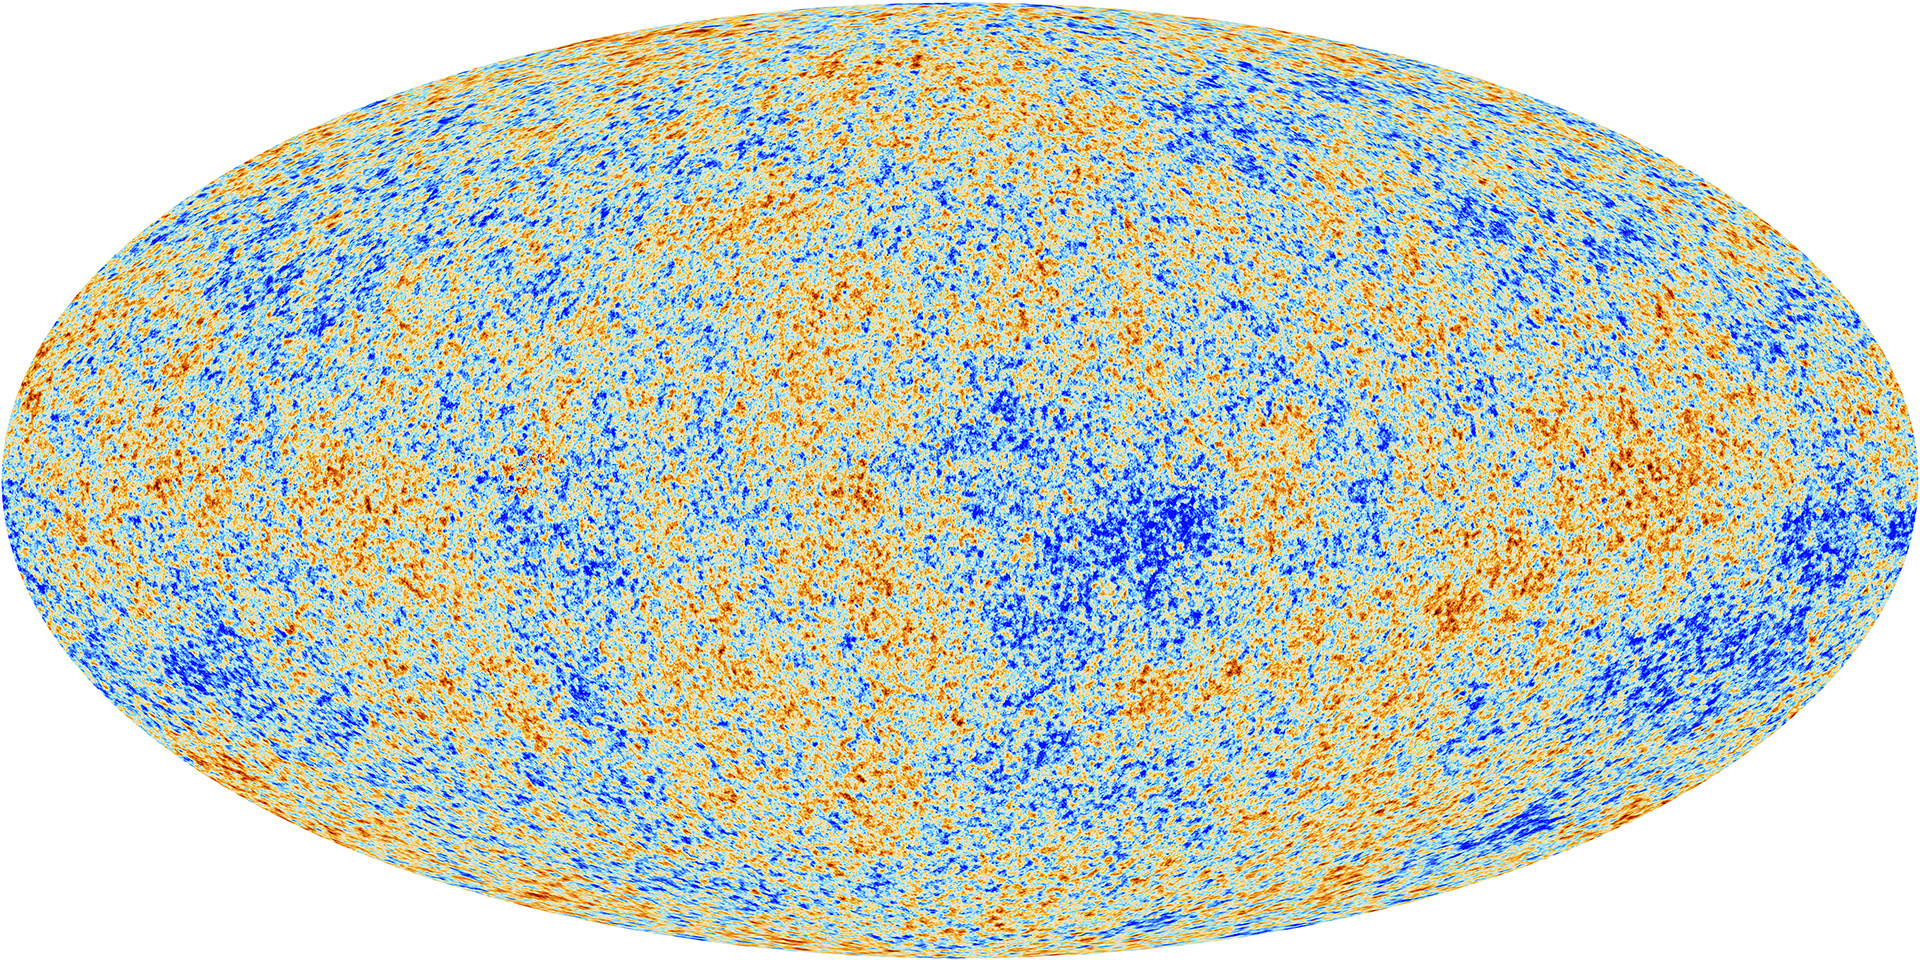
\includegraphics[width=.6\textwidth]{figures/Planck_CMB.jpg}
\end{center}

The \textbf{Cosmic Microwave Background (CMB)} was first discovered by Penzias \& Wilson in 1965 by accident. If the universe is expanding, then at some point in the past hot media would have emitted radiation and cooled to much lower temperatures. The CMB is a isotropic source of radiation that is at a temperature,
\[ T\tsb{CMB} = \SI{2.725 \pm 0.001}{\K} \]
Which was first measured in 1992 by COBE-FIRAS. Recall the blackbody spectrum,
\begin{center}
\begin{tikzpicture}
        \begin{axis}[
            standardplot,
            xmin=0, xmax=10, ymin=0, ymax=2,
            xlabel={$f$},
            ylabel={$\ep_f$},
        ]
        \addplot[domain=0.001:10,smooth,thick, variable=\x,red]  plot ({\x},{\x^3/(e^(\x) - 1)});
        \end{axis}
\end{tikzpicture}
\end{center}

Where $\ep_f$ is the energy of radiation per unit volume per frequency,
\[ \f{\dif E}{ \dif V \dif f} = \ep_f = \f{8\pi h f^3}{c^3\bs{e^{hf/kT} - 1}} \]
Which under appropriate normalization matches the CMB extremely well; making it our most accurate indication for big-bang cosmology. However, there are slight anisotropies in the CMB. The variation in temperature of the CMB is extremely small (discovered COBE-DMR 1992),
\[ \f{\de T}{T} \approx \SI{1e-5}{} \]
For these discoveries, John Marher and G. Smoot shared the Nobel prize in 2006. Since these observations the WMAP (2001) and Planck (2013) projects have obtained higher and higher resolution images of the CMB. \\

In addition to $\mu$-waves, the infrared (IR) spectrum is also important for cosmology. Dust absorbs more and more light at higher and higher frequencies. As such, lower wavelengths are important to be able to see through cosmic dust. As a quick summary, here are some infrared surveys,
\begin{itemize}
    \item 2MASS ($2\mu$, neat IR) stars
    \item IRAS (80's) ($>20\mu$, far IR) dust
    \item Spitzer (new)
\end{itemize}

Moreover X-rays are much more energetic than optical light rays,
\[ E\tsb{optical} \approx \SI{}{\eV} \approx \SI{1.6e-19}{\J} \qquad E\tsb{X} \approx \SI{}{\kilo\eV} \]
The typical temperature of an X-ray is $T\tsb{X} \approx \SI{1e7}{\K}$ which is great for studying clusters of galaxies because most of a clusters mass is in plasma and $T\tsb{plasma} \approx T\tsb{X}$. Clusters are excellent cosmic labs because they are so dense. In fact, our first evidence for dark matter came from studying galaxy clusters via X-rays. \\

Radiowaves are also useful for cosmology because the transition of an electron in a neutral hydrogen atom from spin up to spin down emits weak energy emissions around $\SI{21}{\cm}$. The precision of radiowaves allows one to measure speeds of cosmic bodies by examining shifts in the $\SI{21}{\cm}$ spectrum. The CHIME project is an up-and-coming radiowave telescope.

\subsubsection{Matter in The Universe}

Most of the matter in the universe is made up of particles (with the potential notable exception of dark matter). In truth, the modern perspective on matter is an emergent phenomena of quantum \textit{fields}. From Einstein, we have that,
\[ E^2 = p^2 c^2 + m^2 c^4 \]
Where $E$ is the energy of the particle, $p$ is the momentum and $m$ is the rest mass. If $p \ll m c$ we can take the non-relativistic limit $v = \f{p}{m} \ll c$,
\[ E = \sqrt{p^2 c^2 + m^2 c^4} = mc^2 + \f{1}{2}\f{p^2}{m} + \mathcal{O}\br{m c^2 \f{p^4}{m^4 c^4}} \]
Clearly $\f{1}{2}\f{p^2}{m}$ refers to the standard classical kinetic energy. Higher order corrections to these formulas typically are on the order of $\mathcal{O}\br{c^{-2}}$. On the other hand, for relativistic particles we have that $E \approx pc$ when $v \approx c$. To retain generality, we define the velocity of a particle to be,
\[ \ve{v} = \f{\ve{p}c^2}{E} \]
Here is a breakdown of the contents of the universe: \\
\textbf{Cosmic Content:}
\begin{itemize}
    \item $\%4$ -- baryons/leptons (protons $m\tsb{p} c^2 \approx \SI{}{\giga\eV}$ and electrons $m\tsb{e} c^2 \approx \SI{0.5}{\mega\eV}$)
    \item $\%0.004$ -- radiation (photons $m_{\ga}c^2 = 0$ and neutrinos $m_{\nu}c^2 \approx \SI{0.1}{\eV}$)
    \item $\%25$ -- dark matter (clumpy)
    \item $\%70$ -- dark energy (smooth)
\end{itemize}
The main interactions in the universe are due to photons scattering off of free electrons (\term{Thomas Scattering}) and also weakly interacting neutrinos. We have relative densities,
\[ \rho_{\ga} \approx \rho_{\nu} \approx 10^{-3} \rho_{b} \]
\[ n_{\ga} \approx n_{\nu} \approx 10^{9} n_{b} \]


\subsection{Hubble Law}

The Hubble law (discovered by Hubble) shows that nebulae at further and further distances are moving \textit{away} from us faster and faster. Hubble measured distances (using variable stars) and velocities of spiral nebulae using their Doppler shift (galaxies) using and obtained the following result:
\begin{center}
    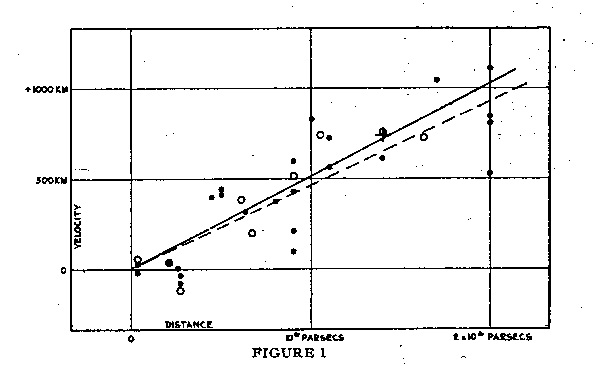
\includegraphics{figures/hubble.jpg}
\end{center}
\[ v_{r} = H r \]
Where $r$ is the distance to the object, $v_{r}$ is the radial velocity of that object and $H$ is a constant known as \term{Hubble's Constant}. Hubble's constant has numerical value,
\[ H = 100 \cdot h \SI{}{\km \per \s \per \mega\pc} \]
Where is a dimensionless number measured to an accuracy $h = \SI{0.68\pm0.02}{}$.
To measure velocities, Hubble used the Doppler shift,
\[ 1+ z = \f{\la\tsb{obs}}{\la\tsb{emit}} = \f{1 + \f{v}{c}}{1 - \f{v}{c}} \]
Where $z$ is called the \term{Redshift} and $v$ is the radial velocity of the object.\footnote{In fact, in a homogeneous universe, the only motion is radial.} As a first order approximation in small $v$,
\[ 1 + z = 1 + \f{v}{c} + \mathcal{O}\bs{\br{\f{v}{c}}^2} \]
In the other limiting case, as $v \to c$, we have that ${\la\tsb{obs}}/{\la\tsb{emit}} \to \inf$ which makes $z \to \inf$.\\

To characterize deviations from Hubble's law, we define the peculiar velocity to be,
\[ \ve{v}_p = \ve{v} - H \ve{r} \]
Where it is typical to have $\ba{v_p^2}^{1/2} \approx \SI{400}{\km\per\s}$. Hubble's law was one of the first indications for the Big-Bang. It fact the time since the big bang is approximately,
\[ t\tsb{big bang} = \f{1}{H} \approx \SI{14}{\giga\yr} \]
Hubble's law gives us a picture of the kinematics of the universe.

\section{Newtonian Cosmology}

Now that we have a rough idea of the contents and kinematics of our universe, we shall start to study the dynamics of the universe. In doing so, we will approach an obstacle; as we look at farther and farther objects, Hubble's law dictates that these objects are moving faster and faster. At some point these objects are moving \textit{faster} than the speed of light. As such, in order to do justice to Cosmology, one should study it through the lens of general relativity.\\

Despite this, we can take a shortcut ($\Phi_N = - {GM}/{r}$).
\[ \abs{\Phi_{N}}, v^2 \ll c^2 \quad \text{vs.}\quad \abs{\Phi_{N}}, v^2 \approx c^2 \]
To study local properties of the universe, it is sufficient to use Newtonian physics. Of course, global properties require a relativistic treatment. As such we will first focus on Newtonian Cosmology.\\

Consider two spherical\footnote{Objects that are not spherical exhibit deviations from \cref{eq:next_grav} known as \term{tidal forces}.} masses $M$ and $m$ and the force between them,
\[ F = \f{G M m}{r^2} \eq \label{eq:next_grav} \]
As well as the potential energy,
\[ V = m \Phi_N = -\f{GMm}{r} \]
Another thing of note is that masses are always positive $m \geq 0$. To contrast Newton, the most important equation in Cosmology is the \term{Friedmann equation}. If the universe is homogeneous we can pick a generic point to be the origin for the universe and define a ball of radius $r$ (growing at rate $\dot{r}$) around this point enclosing a mass $M = \f43 \pi r^3 \rho$. By conservation of energy,
\begin{align*}
U &= T + V = \text{const.} \\
&= \f{1}{2} m \dot{r}^2 - \f{GMm}{r} \\
&= \f{1}{2} m \dot{r}^2 - \f43 \pi \rho G m r^2 \eq \label{eq:conser_fried_eq}
\end{align*}
Next define a \term{co-moving} coordinate $\ve{x}$ such that $\ve{r}\br{\ve{x}, t} = a\br{t} \ve{x}$. For each particle at $\ve{x}$, as the universe expands, $\ve{x}$ follows the location of the particle. The physical coordinate of the particle is $\ve{r}$ and the relevant dimensionless scale factor is $a\br{t}$. These concepts hold for all ``origins'' provided that the universe is homogeneous and isotropic. Substituting the co-moving coordinate into \cref{eq:conser_fried_eq} yields the Friedmann equation,
\[ \br{\f{\dot{a}}{a}}^2 = \f{8 \pi G}{3} \rho_b - \f{k c^2}{a^2} \eq \label{eq:friedmann_equation} \]
Where $k$ is defined such that,
\[ k c^2 = - \f{2 U\br{x}}{m x^2} \]
In order for the universe to remain homogeneous, it must be that $k$ does not depend on $x$. Therefore $k$ is a constant in a homogeneous universe. By dimensional analysis on \cref{eq:friedmann_equation} it can be seen that $k$ has dimensions $\text{length}^{-2}$. In general relativity $k$ becomes the curvature of the space. Intuitively, a homogeneous universe has the same curvature everywhere. \\

One misconception associated with the expansion of the universe is that \textit{everything} in the universe is expanding. However, object that are close enough can be bound together by interactions in various fields. As such, the expansion of the universe has little to no observable affect on local objects like planets or people or galaxies. \\

\subsection{Solving the Friedmann Equation}

Solving the Friedmann equation corresponds to solving \cref{eq:friedmann_equation} together with the \term{fluid equation}. The fluid equation comes from the first law of thermodynamics ($\dif E + p \dif V = T \dif S = 0$), which translates to,
\[ E = \pi a^3 x^3 \rho c^2 \qquad V = \f43 \pi a^3 x^3 \]
Which gives the continuity equation,
\[ \dot{\rho} + \f{3\dot{a}}{a} \br{\rho + \f{P}{c^2}} = 0 \eq \label{eq:fluid}\]
Where the pressure $P\br{\rho}$ is determined by the equation of state. Combining \cref{eq:fluid} and \cref{eq:friedmann_equation} gives,
\[ \f{\ddot{a}}{a} = - \f{4 \pi G}{3} \br{\rho + \f{3P}{c^2}} \]
Which is a relativistic manifestation of Newton's law. The difference being the term term involving pressure $P$.

\section{Geometry}

\begin{center}
\begin{tabular}{|c|c|}
    \hline
    Geometry & k \\
    \hline
    Hyperbolic & -1 \\
    Flat & 0 \\
    Geometry & +1 \\
    \hline
\end{tabular}
\end{center}
\todo[TC]{Clean up this lecture}
\[ \ell = \begin{cases}
    \phi R \sin\br{\f{r}{R}} & k = +1 \\
    \phi r & k = 0 \\
    \phi R \sinh\br{\f{r}{R}} & k = -1 \\
\end{cases} \]
Introduce the spacial components of the \term{Friedmann Robertson Walker (FRW) metric},
\[ \dif s^2 = a^2\br{t}\br{\f{\dif r^2}{1 - kr^2} + r^2 \br{\dif \theta^2 + \sin^2 \theta \dif \phi^2}} \eq \label{eq:FLRW}\]
There is a choice in dimensionality among the terms involved. Typically, $a\br{t}$ is taken to be a dimensionless quantity such that $r$ and $k$ have units. In doing so, we can make the scaling choice of,
\[ a\br{t\tsb{now}} = a\br{t_0} = a_0 \defined 1 \]
Where $t_0$ is used to denote the present time. Therefore $r$ has units of length and $k$ necessarily has units of $\text{length}^{-2}$. Considering the different possibilities for $k$ ($\bc{k < 0, k = 0, k > 0}$), observational data has not been able to distinguish the curvature $k$ of our universe. Experiments suggest it is close to zero. \\

Recall that for an isotropic expansion, we need $a\br{t}$ on the ``outside'' of \cref{eq:FLRW} and so $r,\theta,\phi$ (or $x,y,z$ in flat space) are commoving coordinates. We will also see that galaxies have $r, \theta, \phi$ approximately fixed (in a homogeneous universe).\\

\textit{What is the velocity of a galaxy?} Obviously velocity is the derivative of a distance. However there are many different distances to consider in cosmology. One option is to define the distance between two objects at a fixed time called \term{proper time}. To calculate proper time take $\dif s^2$ at fixed time $t$ and integrating over $\dif r$ and setting $r=0$ to be the reference galaxy. Integrating along a radial line $\dif \phi = \dif \theta = 0$. Thus,
\[ d\tsb{prop} = a\br{t} \underbrace{\intl_{0}^{r} \f{\dif r'^2}{\sqrt{1 - k r'^2}}}_{\chi} \]
Note that for a galaxy, if $r$ is constant then $\chi$ is constant as well.
The \term{proper velocity} in this case is of course,
\[ \dot d\tsb{prop} = \dot a \chi = \dot a \f{d\tsb{prop}}{d} = \br{\f{\dot a}{a}} d\tsb{prop} \]
Which is identical to Hubble's law,
\[ \bc{\dot r = H_0 r} \sim \bc{\dot d\tsb{prop} = \br{\f{\dot a}{a}} d\tsb{prop}}  \]
Therefore it could be that Hubble's constant is a function of time,
\[ H\br{t} = \f{\dot a}{a} \eq \label{eq:hubble_scale_factor} \]
\subsection{Summary of General Relativity}
Without delving into the rigor and formalism of General Relativity, we summarize some of the ideas behind the foundations of GR.\\

The \term{equivalence principle} is best introduced via an analogy to electrostatics. In electrostatics, the force between two charges $Q, q$ is,
\[ F = \f{1}{4\pi\ep_0}\f{Qq}{r^2} \]
Therefore the acceleration on the smaller charge $q$ with mass $m$ is,
\[ a = \f{Qq}{4\pi\ep_0mr^2} = \f{Q}{4\pi\ep_0r^2}\br{\f{q}{m}} \]
Quite characteristically, the acceleration depends on the ratio $q/m$. Therefore an electron and proton will have a very different acceleration when nearby the same charge $Q$. In contrast, gravity behaves \textit{differently}. In gravity,
\[ F = \f{GMm}{r^2} = ma \]
Therefore,
\[ a = \f{GM}{r^2} \br{\f{m}{m}} = \f{GM}{r^2} \]
Therefore any object (regardless of its mass) has the same acceleration; hinting at the fact that gravity is \textit{special}. The equivalence of $m\tsb{grav}$ and $m\tsb{inert}$ then suggests the famous elevator thought experiment. Because of the mass equivalence, no experiment can distinguish the difference between an experiment on earth (in a uniform gravitational field) and a uniform acceleration (like in a rocket). Therefore, if the light from a laser in a rocket appears to bend downward in a rocket (due to the acceleration) it must also be the case that light bends downward toward earth! The resolution between this thought experiment and Fermat's optical principle is that space itself is bending in a gravitational field. The light in a gravitational field follows ``straight'' \term{geodesics}. Freely-falling objects (particles, photons) follow geodesics in space-time. \\

There is an important caveat to the equivalence principle. If the rocketships (elevators) has size comparable to the size of the earth, then the body will experience forces in different directions across its extent in a gravitational field but \textit{not} when uniformly accelerating. These forces are known as \term{tidal forces}. So in Gr space time must behave like special relativity on small scales. In SR the spacetime line element is written as,
\[ \dif s^2 = - c^2 \dif t^2 + \dif x^2 + \dif y^2 + \dif z^2 \]
Photons taking at speed $c$ has the defining property that,
\[ \dif s^2_\ga  = 0 \eq \label{eq:null_geodesics}\]
Which can be stated as: \textit{photons travel on null geodesics}. Therefore the \term{full FRW metric} must be,
\[ \dif s^2 = - c^2 \dif t^2 + a^2\br{t}\br{\f{\dif r^2}{1 - kr^2}} + r^2 \br{\dif \theta^2 + \sin^2 \theta \dif \phi^2} \eq \label{eq:FRW_full}\]
To solve for the equations of motion or geodesics of photons, one simply needs to solve \cref{eq:FRW_full} under the constraint that \cref{eq:null_geodesics}. In summary the following comparison holds,
\begin{center}
\begin{tabular}{|l|l|}
    \hline
    Special Relativity & General Relativity \\
    \hline
    Special observers are inertial & Freely falling \\
    Light follows null geodesics & same \\
    Particles move in straight lines & Particles follow geodesics \\
    Empty universe / No curvature & Not empty universe / Curvature \\
    \hline
\end{tabular}
\end{center}
Note that the ``flat'' universe $(k=0)$ is spatially flat, but curved in space-time. \\

\subsection{Einstein Equation}

The Einstein equation relates functions of the metric $(\dif s^2 = \cdots)$ to the energy content of the universe. Typically, the Einstein equations are $10$ non-linear equations. When applied to a homogeneous universe (as is considered in cosmology), the Einstein equations reduce to $2$ equations. One of which is the Friedmann equation,
\[ \br{\f{\dot a}{a}}^2 + \f{k c^2}{a^2} = \f{8 \pi G}{3} \rho \]
Where $kc^3/a^2$ is related to the energy content but here it is related to the curvature as well (same $k$ as in FRW metric).

\end{document}